\documentclass[11pt,a4paper]{article}

\usepackage[margin=2.5cm]{geometry}
\usepackage{booktabs}
\usepackage{tabularx}
\usepackage{array}
\usepackage{amsmath}
\usepackage{hyperref}
\usepackage{microtype}
\usepackage{parskip}
\usepackage{enumitem}
\usepackage{caption}
\usepackage{float}
\usepackage{xcolor}
\usepackage{titlesec}
\usepackage{graphicx}

\hypersetup{
    colorlinks=true,
    linkcolor=black,
    urlcolor=blue,
    citecolor=black
}

\titleformat{\section}{\large\bfseries}{\thesection}{1em}{}
\titleformat{\subsection}{\normalsize\bfseries}{\thesubsection}{1em}{}

\title{\textbf{Data Mining Assignment 3}\\[0.3em]
       \large Clustering and Anomaly Detection on a Mixed Article Dataset}
\author{Samuel van Nimwegen}
\date{1 May 2026}

\begin{document}

\maketitle

\noindent\textbf{GitHub repository:}
\url{https://github.com/samuelvnimwegen/data-mining-anomaly-detection.git}

\bigskip

\section{Task 1: Data Exploration and Preprocessing}

\subsection{Dataset overview}

The dataset contains \textbf{2,164 documents} stored in \texttt{articles.csv}. Each document is a short newsgroup discussion article. Based on the newsgroup source, we expected to find topic groups such as medicine, computing, space and science, sports, and automotive discussions, along with a small number of spam or corrupted files. Text length varies widely, with an average of \textbf{886 characters} and around \textbf{160 words} per document. A random sample confirmed these expectations: 82 documents contained HTML markup and 136 showed unusually high symbol density, suggesting that some documents are structurally unusual.

\subsection{Preprocessing pipeline}

Because clustering and anomaly detection need different types of information, a \textbf{two-view normalisation} approach was used, producing two parallel versions of each document.

The \textbf{clustering view} applies aggressive cleaning: HTML, URLs, digits, and punctuation are removed, text is lower-cased, stop-words are removed (NLTK), and tokens are lemmatised with spaCy. Rare tokens (document frequency $< 1$) and very common tokens (document frequency $> 92\%$) are also removed. After this step, the vocabulary shrank from 345,517 to 160,129 tokens (a 54\% reduction). The cleaned texts were vectorised with TF-IDF (unigrams and bigrams, 20,000 features). A bag-of-words matrix (unigrams, 20,000 features) was also built from the clustering view and saved to \texttt{data/results/bag\_of\_words\_matrix.csv} as the Task~1 deliverable.

The \textbf{anomaly view} keeps punctuation, digits, and casing, preserving repetition and formatting patterns that signal unusual documents. Two feature sets were built from this view: (i) a character $n$-gram TF-IDF matrix (3 to 5-grams, 30,000 features) compressed to 256 dimensions via LSA, and (ii) \textbf{17 hand-crafted structural features} described in Section~\ref{sec:task3}.

\section{Task 2: Clustering}
\label{sec:task2}

\subsection{Methods and experimental design}

Two feature representations were compared across $k \in \{2, \ldots, 10\}$ using three algorithms. \textbf{TF-IDF} provides a sparse word unigram/bigram matrix (20,000 features). \textbf{Sentence embeddings} are dense 384-dimensional vectors from \texttt{all-MiniLM-L6-v2}, which encode semantic meaning rather than surface word overlap. The three algorithms were \textbf{K-Means} (Euclidean distance, \texttt{random\_state=42}), \textbf{Agglomerative} (Ward linkage, which minimises within-cluster variance at each merge step and tends to produce more balanced cluster sizes than single or complete linkage), and \textbf{Spectral} (RBF affinity kernel). Quality was measured with the \textbf{silhouette score}. A \textbf{size constraint} was added: the largest cluster must not exceed 1,300 documents (60\% of the dataset).

\subsection{Results and cluster interpretation}

Table~\ref{tab:clustering} summarises the main results. Spectral clustering always violates the size constraint (the RBF kernel collapses most documents into one group) and was removed from consideration. TF-IDF clustering is hurt by the curse of dimensionality: cluster borders become unclear in the high-dimensional sparse space, and the best TF-IDF result (Agglomerative $k=8$, silhouette 0.053) has a very uneven size distribution with one cluster of 1,124 documents and others with only 3 to 7. Sentence embeddings fix this by encoding semantic meaning in a dense space. Every embedding configuration scores higher than any TF-IDF alternative, with much more balanced cluster sizes (50 to 564 documents).

\textbf{Effect of cluster count.} Increasing $k$ from 5 to 8 splits the largest general-discussion group into more specific topics: Automotive and General discussion separate into their own clusters, and a distinct Food \& diet group emerges. Below $k=5$ the promotional spam documents begin to merge with general discussion, losing the clean isolation visible in Cluster~4. Above $k=8$ the silhouette score drops and small clusters of fewer than 30 documents appear, which are too small to represent a meaningful topic. $k=8$ gives the best balance between topic detail and cluster stability.

Embedding K-Means $k=8$ (silhouette 0.062) was chosen for the submission over $k=5$ (silhouette 0.065) because it recovers finer topic groups.

\begin{table}[H]
\centering
\caption{Selected clustering results. \checkmark~= passes size constraint ($\leq 1300$ documents). Best valid solution highlighted.}
\label{tab:clustering}
\begin{tabular}{llrrr}
\toprule
Method & $k$ & Silhouette & Max cluster & Passes constraint \\
\midrule
\textbf{Embedding + K-Means} & \textbf{5}  & \textbf{0.065} & \textbf{510}  & \checkmark \\
Embedding + K-Means          & 8  & 0.062 & 397  & \checkmark \\
Embedding + Agglomerative    & 6  & 0.058 & 564  & \checkmark \\
TF-IDF + Agglomerative       & 8  & 0.053 & 1124 & \checkmark \\
TF-IDF + Agglomerative       & 7  & 0.069 & 1629 & $\times$ \\
TF-IDF + K-Means             & 8  & 0.013 & 866  & \checkmark \\
TF-IDF + Spectral            & 9  & 0.092 & 2015 & $\times$ \\
\bottomrule
\end{tabular}
\end{table}

\begin{figure}[H]
\centering
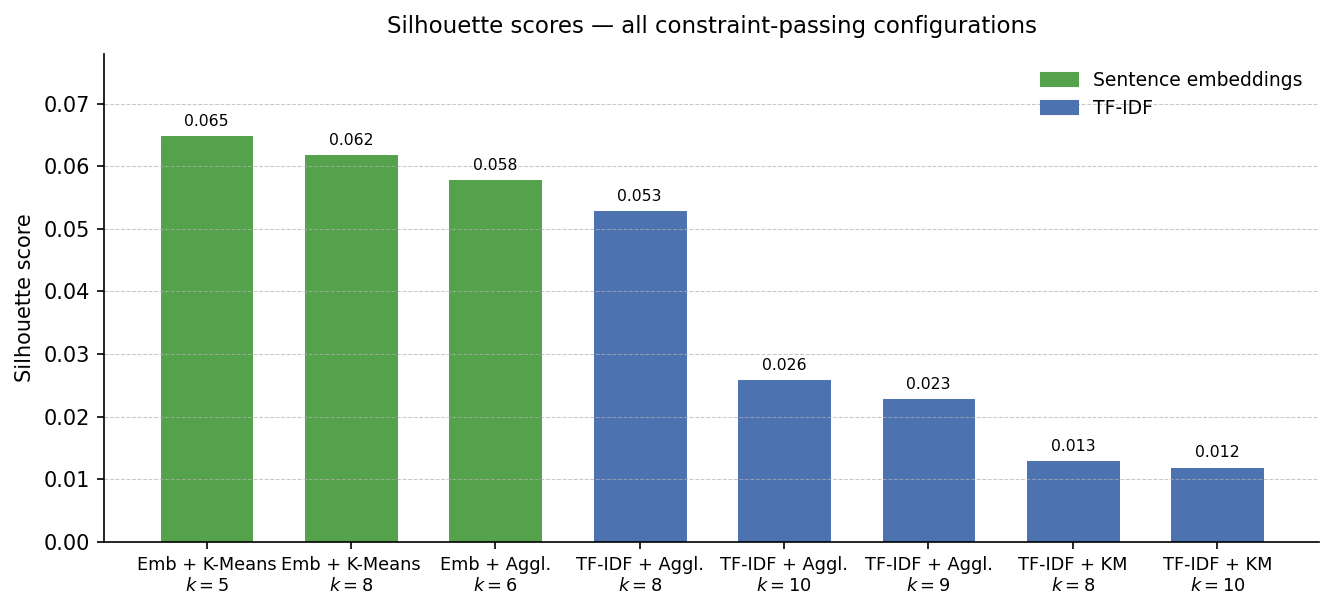
\includegraphics[width=0.85\textwidth]{report_figures/fig1_silhouette_comparison.pdf}
\caption{Silhouette scores for all configurations that pass the size constraint. Spectral clustering is omitted.}
\label{fig:silhouette}
\end{figure}

Table~\ref{tab:kmeans} shows the eight clusters from the chosen solution. All clusters match recognisable newsgroup categories. One thing worth noting: a basic TF-IDF check of Cluster~0 shows terms like \textit{gordon bank} and \textit{chastity}, which look like spam. These come from a recurring email signature used by a frequent medical-newsgroup poster. The sentence embeddings are not affected by this and correctly group these documents as medical discussions, which shows the advantage of dense representations over bag-of-words. The known anomalies are strongly concentrated: 41 of the 50 flagged documents are in Cluster~4 (Promotional spam), confirming that clustering and anomaly detection capture the same signal.

\begin{table}[H]
\centering
\caption{Embedding K-Means $k=8$ clusters: sizes and top centroid terms.}
\label{tab:kmeans}
\begin{tabularx}{\textwidth}{clrX}
\toprule
Cluster & Inferred topic & Docs & Top content terms \\
\midrule
0 & Medicine \& health             & 307 & doctor, patient, disease, pain, medical, treatment \\
1 & Automotive                     & 374 & car, engine, dealer, price, good \\
2 & Graphics \& computing          & 340 & file, graphic, program, image, format, window \\
3 & Space \& science               & 236 & space, moon, launch, nasa, orbit, lunar \\
4 & Promotional spam               &  50 & ref, promo, sale, id, offer, code \\
5 & General discussion             & 362 & just, like, think, point, time, know \\
6 & Sports (hockey)                & 397 & game, team, hockey, player, play, playoff \\
7 & Food \& diet                   &  98 & food, msg, taste, cause, chinese, diet \\
\bottomrule
\end{tabularx}
\end{table}

To go beyond the numerical score, the nearest-centroid document was selected per cluster as a representative example. Cluster~6's representative document discusses NHL playoff scheduling. Cluster~3's representative concerns the cost justification of lunar missions. Cluster~7's representative debates food poisoning causation. Cluster~4's representative is a short promotional listing with repeated offer codes, which matches the top terms exactly. These examples confirm that the clusters capture real topic groups and are not the result of noise or artefacts.

\begin{figure}[H]
\centering
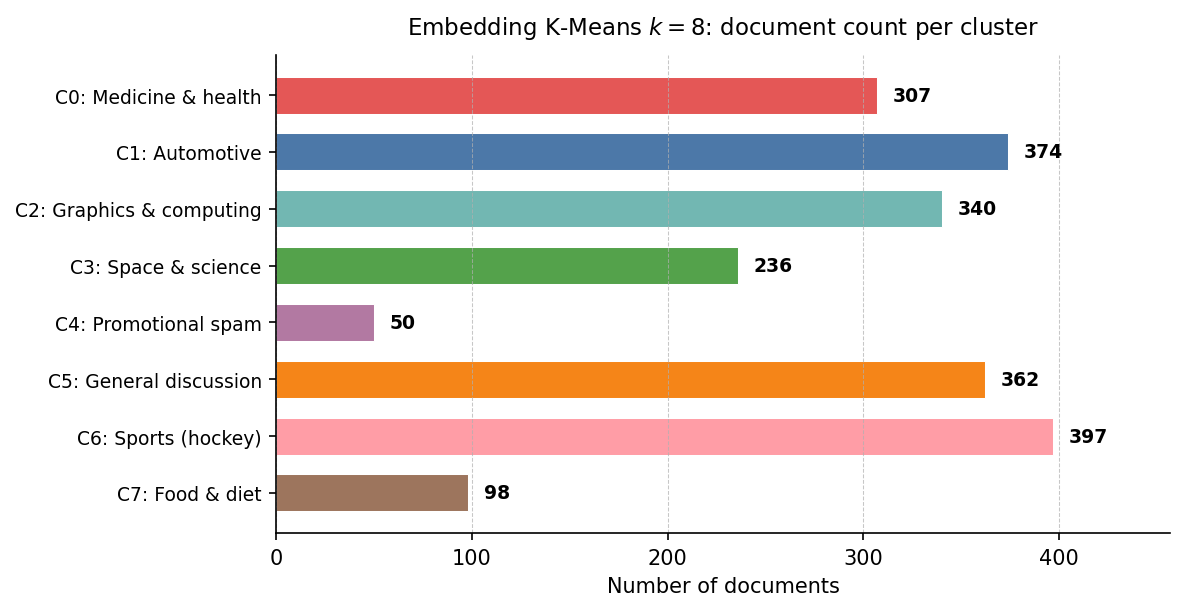
\includegraphics[width=0.85\textwidth]{report_figures/fig2_kmeans_cluster_sizes.pdf}
\caption{Document counts per cluster for the $k=8$ solution (50 to 397 documents per cluster).}
\label{fig:clustersizes}
\end{figure}

\begin{figure}[H]
\centering
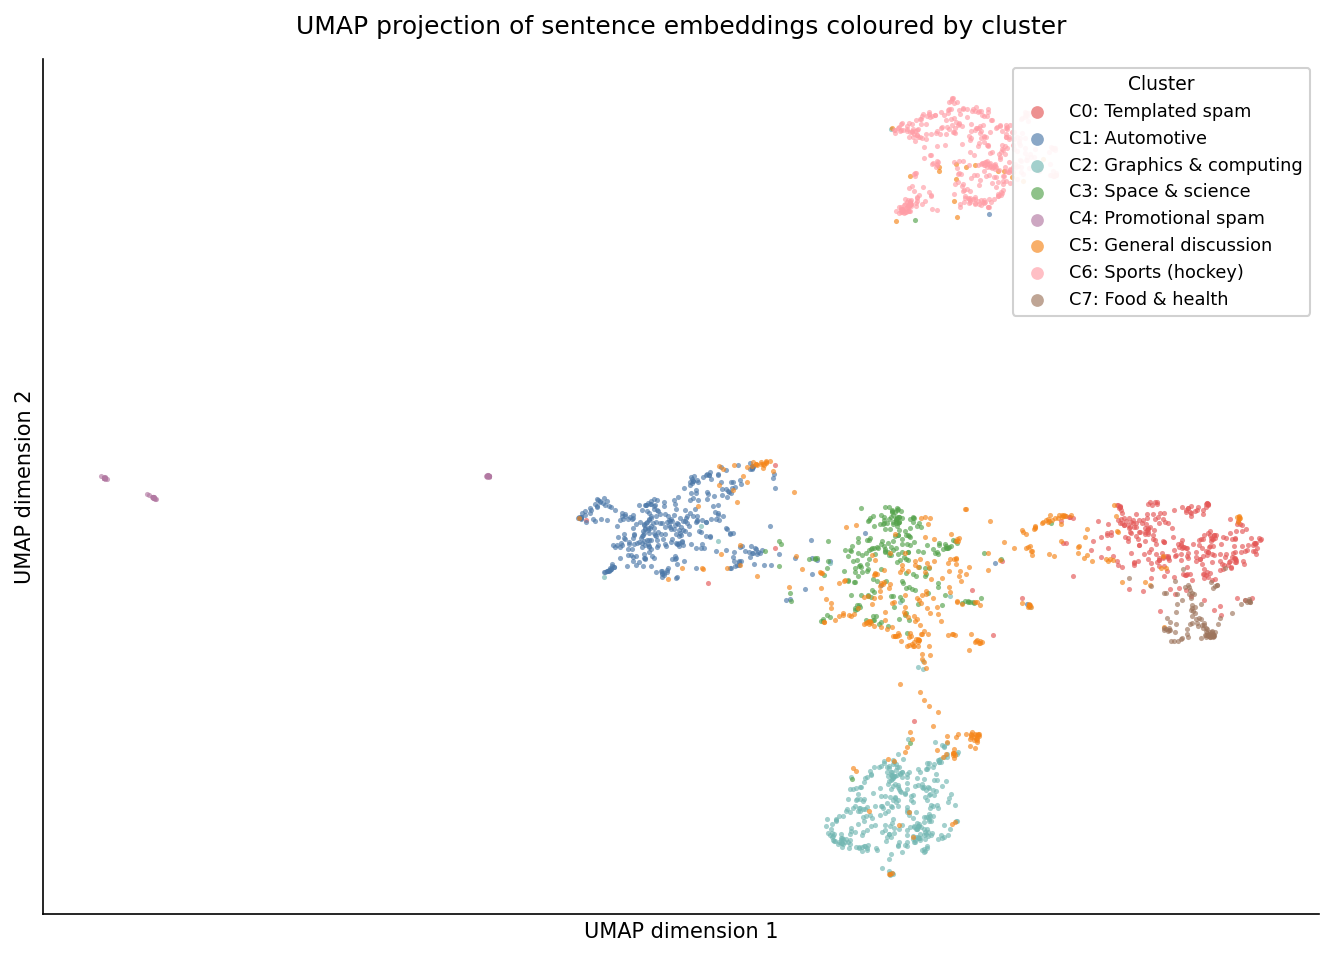
\includegraphics[width=0.85\textwidth]{report_figures/fig3_umap_clusters.pdf}
\caption{UMAP projection of the 384-dimensional sentence embeddings coloured by cluster. Spam clusters (C4) are clearly isolated. Graphics (C2) is compact and well-separated. General discussion (C5) sits in a transition zone between Sports and Automotive, as expected for a mixed-topic category.}
\label{fig:umap}
\end{figure}

\section{Task 3: Anomaly Detection}
\label{sec:task3}

\subsection{Feature engineering}

Text anomalies from unusual formatting and repetition are not well captured by semantic features. A set of \textbf{17 structural surface features} was created, covering: \textbf{length} (character count, token count, average token length), \textbf{vocabulary} (type-token ratio, repeated-token ratio, max repeated-token run, lexical entropy, bigram type-token ratio), \textbf{character-class ratios} (uppercase, digit, punctuation), \textbf{special patterns} (URL count, email count, HTML tag count, mixed alphanumeric ratio, placeholder ratio), and \textbf{compression ratio} (compressed size / original size), a direct measure of textual repetition. The structural feature matrix has shape $(2164, 17)$.

\subsection{Methods and results}

Three detectors were applied to the structural feature matrix. \textbf{Isolation Forest (IF)} uses contamination 2.3\% and scores documents by how easily they are isolated in random trees. \textbf{Local Outlier Factor (LOF)} uses $k=20$ neighbours and scores by relative local density. \textbf{kNN} uses the mean distance to the 10 nearest neighbours.

Table~\ref{tab:overlap} shows the pairwise top-50 overlap. IF and LOF agree on 22 of 50 (44\%). kNN diverges strongly, sharing only 2 documents with each of the others. The reason is the \textbf{clustered anomaly problem}: the 50 anomalous templated documents are close to each other, so their average neighbour distance is \emph{low}. kNN therefore ranks them as normal and flags isolated legitimate documents instead. LOF is less affected but has the same issue. Isolation Forest is not fooled because it measures isolation depth, not distance.

Semantic features (TF-IDF and LSA) were also tested with Isolation Forest. The Spearman correlation between their rankings was $\mathbf{-0.131}$, with only 4 shared candidates in the top 50, confirming that the anomalous documents differ in \emph{structure}, not vocabulary.

\begin{table}[H]
\centering
\caption{Pairwise top-50 overlap between anomaly detection methods (structural features).}
\label{tab:overlap}
\begin{tabular}{lr}
\toprule
Method pair & Top-50 overlap \\
\midrule
IF vs.\ LOF & 22 / 50 \\
IF vs.\ kNN & 2 / 50 \\
LOF vs.\ kNN & 2 / 50 \\
\bottomrule
\end{tabular}
\end{table}

\subsection{Final anomaly list}

Isolation Forest on the 17 structural features was chosen as the main detector. The 50 top-ranked documents were saved to \texttt{anomalies.csv}. The separation is clear: anomaly median compression ratio is 0.43 versus 0.63 for normal documents, and anomaly median repeated-token ratio is 0.83 versus 0.42. Figure~\ref{fig:anomalyfeatures} confirms this across four features. The top candidates include documents made of a single repeated phrase (e.g.\ ``fast deal fast deal\ldots''), dense promotional text with markup fragments, and heavily quoted reply chains with high punctuation ratios.

\begin{figure}[H]
\centering
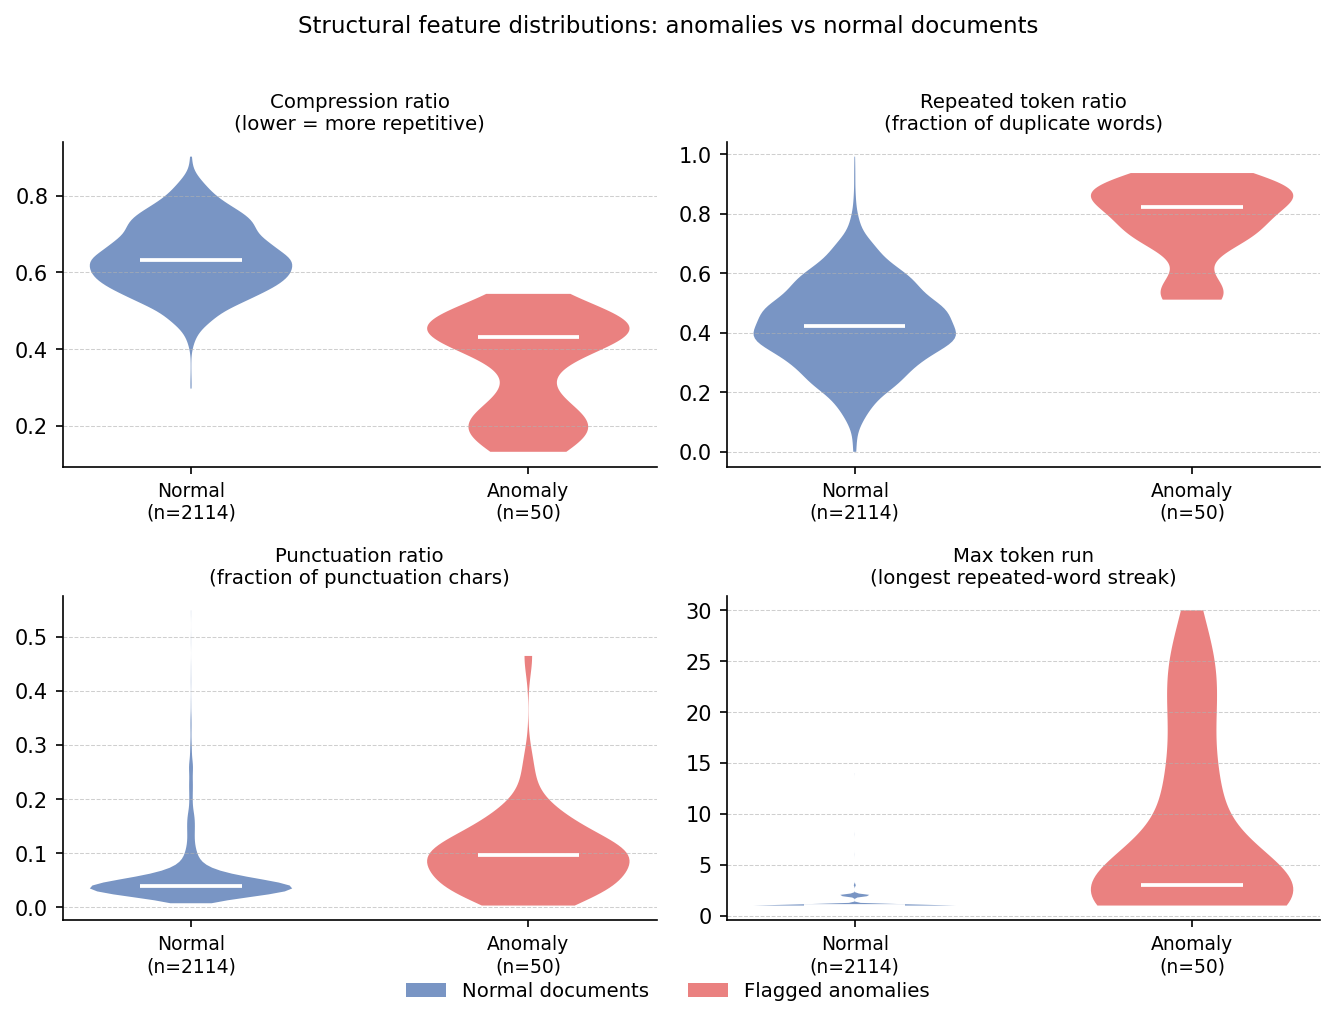
\includegraphics[width=0.85\textwidth]{report_figures/fig4_anomaly_features.pdf}
\caption{Violin plots comparing four structural features for the 50 anomalies (red) versus 2,114 normal documents (blue). Anomalies have lower compression ratios, higher repeated-token ratios, higher punctuation ratios, and much larger max token runs (capped at 30 for display).}
\label{fig:anomalyfeatures}
\end{figure}

\section{Conclusion}

For clustering, sentence embeddings (\texttt{all-MiniLM-L6-v2}) perform much better than TF-IDF across all methods tested. The final submission uses Embedding K-Means $k=8$ (silhouette 0.062), which finds eight clear topic groups. The UMAP projection confirms that these groups are well separated. For anomaly detection, Isolation Forest on 17 structural features outperforms distance-based methods (kNN, LOF) and semantic methods (TF-IDF, LSA). The violin plots give clear evidence: the 50 flagged documents are separated from the 2,114 normal documents on every structural measure used.

\end{document}
